\section{Implementation}
\subsection{CPU variant}
The most computationally involved step of the PM method is the potential solver.
As explained in \autoref{sec:solving-the-field-equation}, in our implementation, we solve the Poisson equation for the potential using the convolution method.
This approach involves taking the DFT of the grid-defined density and later the inverse DFT of the product of transformed Green's function and the transformed density.
Since the number of grid points in a typical grid can be of the order of a million, employing a well-optimized implementation of the FFT is of paramount importance.
We attempted to incorporate a handful of popular C++ FFT libraries into the program, and out of those considered, FFTW \cite{FFTW05} and kissfft \cite{kissfft} provided the best performance.
The running times for FFT and inverse FFT stages of the algorithm using each of the libraries are shown in \autoref{fig:cic-shape}.
\begin{figure}[htp]
    \centering
    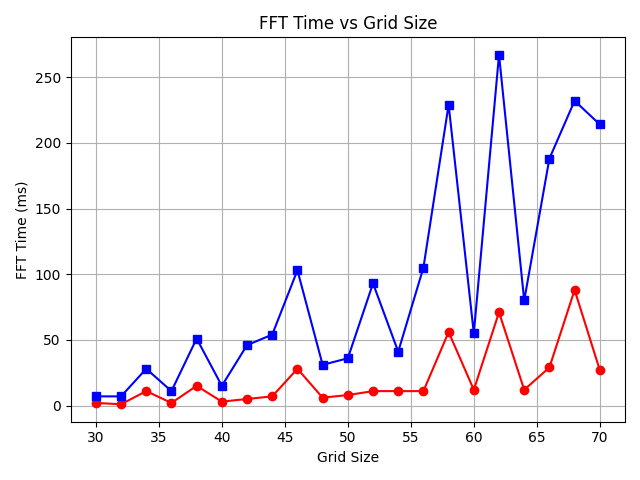
\includegraphics[scale=0.5]{chapters/pm-method/img/fft_time.png}
    \caption{Time needed to perform the DFT and inverse DFT using kissft (red, round markers) and FFTW (blue, square markers) libraries.
        The total grid size in the test was $(2N_g)\times (2N_g) \times N_g$, where $N_g$ is labeled as ``Grid Size'' on the horizontal axis in the graph.}
    \label{fig:fft-time}
\end{figure}
As we can see, FFTW considerably outperformed kissfft, with the former achieving an average five-fold speedup over the latter.

As noted in \autoref{sec:mass-assignment}, parallelization of the mass assignment step, which involves ``spreading'' the mass due to a particle over nearby cells, requires synchronization to avoid data races.
The above requirement can be fulfilled by using mutexes or atomic operations.
Traditionally, atomic RMW operations were supported by the C++ standard library only for the integer types; however, recently, C++20 introduced atomic RMW operations on floating point numbers (see \url{https://en.cppreference.com/w/cpp/atomic/atomic.html}).
We conducted a simple benchmark on Intel Core i7-9750H CPU (three threads concurrently incrementing a global variable) to compare the performance of both approaches.
The benchmark indicated that guarding the critical section with a mutex was around two times faster than using atomic operations.
However, the same test run on a system with a different processor indicated that using an atomic counter offers better performance, suggesting that more careful benchmarking would be needed to reach a definitive conclusion.
In any case, in our implementation we decided to use mutexes for synchronization.

\subsection{GPU variant}\label{subsec:gpu-variant}
As explained before, the mass assignment, field calculation at mesh points, and interpolation steps of the PM method are embarrassingly parallel.
For this reason, rewriting the PM code for the GPU does not pose much difficulty.
In our implementation, we used CUDA C++ language extension to implement the method on the GPU.
A thorough introduction to the arcana of programming NVIDIA GPU devices is given in \cite{nvidia2025cuda}.
In this work, we only remark on the aspects directly related to our use case.

The memory hierarchy of a GPU (also referred to as the \textit{device}) is organized into three main levels:
\begin{enumerate}
    \item global memory (accessible by all threads as well as \textit{host} (CPU); high latency),
    \item shared memory (accessible by threads in the same threadblock typically up to 48 KB; very low latency),
    \item local storage (per thread storage in the form of registers managed by the compiler).
\end{enumerate}
One step of the PM method that could potentially benefit from transferring data to shared memory is the gradient calculation step.
For example, if the 2-point finite difference approximation to the Laplacian is used, the potential from six cells needs to be fetched from memory.
At the same time, there is an overlap between the potential data read by threads working on adjacent mesh cells.
Thus, fetching the potential data into shared memory could have a positive impact on performance.
However, our tests for the 2-point approximation, performed at the early stages of the program's development, did not indicate a significant improvement in the algorithm's running time, and this optimization path was not explored further.

A significant performance bottleneck in the GPU implementation is the transfer of data between the host and the device.
These data transfers are necessary if one wishes to record the state of the simulation after each timestep.
However, assuming that only the final state of the simulation is of interest, the PM method can execute entirely on the device, transferring the data to the host only once after the final iteration of the simulation.
This is the scenario that we assumed to compare the CPU and GPU implementation.
The results of the test for different particle numbers are shown in \autoref{fig:cpu-vs-gpu-pm}.
\begin{figure}[htp]
    \centering
    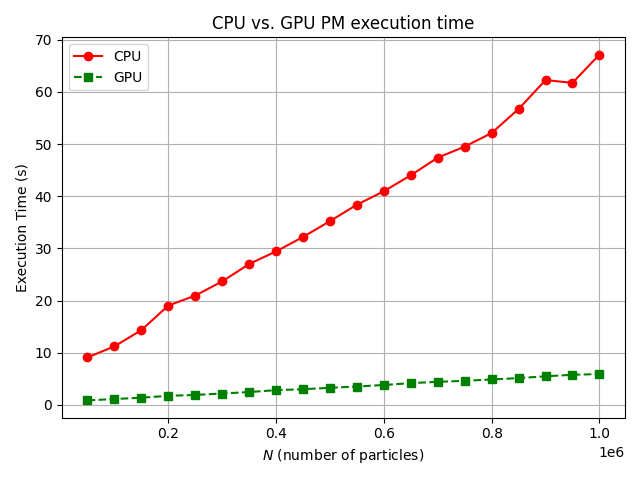
\includegraphics[scale=0.6]{chapters/pm-method/img/cpu-vs-gpu.png}
    \caption{PM method: CPU and GPU implementation running time comparison (200 iterations; intermediate state not saved).}
    \label{fig:cpu-vs-gpu-pm}
\end{figure}
In the test, the computational domain was split into $64\times 64 \times 32$ cells, and the simulation was run for 200 iterations.
Both plots in the figure exemplify the linear complexity of the PM method, with the GPU implementation providing 1200\% speedup over the CPU version.